\documentclass[preprint]{sigplanconf}

\usepackage{tabularx}
\usepackage{amsfonts}
\usepackage{amsmath}
\usepackage{natbib}
\usepackage{graphicx}
\usepackage{tikz}
\usepackage{mathtools}
\usetikzlibrary{chains,fit,shapes,calc}
\usepackage{verbatim}
\usepackage{semantic}
%%\usepackage{DejaVuSansMono}
%%\usepackage{fontspec}
\usepackage{tabu}
\usepackage{amsthm}
\usepackage{mathptmx}
\usepackage{todonotes}
\usepackage{listings, lstcoq}
\usepackage{ucs}
\usepackage[utf8x]{inputenc}
\lstset{language=Coq,
        inputpath=code
       }
\newcommand{\concat}{\ensuremath{+\!\!\!\!+\,}}  

\newtheorem{theorem}{Theorem}[section]
\newtheorem{corollary}{Corollary}[theorem]
\newtheorem{lemma}[theorem]{Lemma}

\begin{document}

\conferenceinfo{ICFP 2018}{} 
\copyrightyear{2018} 
\copyrightdata{[to be supplied]} 

\titlebanner{Preprint}        % These are ignored unless

\title{Verifiably Lazy}
\subtitle{Verified Compilation of Call-by-Need}

\authorinfo{George Stelle}
           {University of New Mexico}
           {stelleg@cs.unm.edu}
\authorinfo{Darko Stefanovic}
           {University of New Mexico}
           {darko@cs.unm.edu}
\maketitle

\begin{abstract}
We present a verified compiler that preserves call-by-need semantics when
compiling lambda calculus into a simple assembly language. We use a recently
developed abstract machine that implements call-by-need semantics using shared
environments to implement and reason about the compiler. We show that the
abstract machine ensures that the compiled assembly code implements a
call-by-need natural semantics. In addition to the standard proof of correct
results, we prove time complexity is preserved, ensuring that memoization.
Because call-by-need is an optimization for call-by-name, we also show the
$\beta$ reduction semantics of call-by-name are preserved.
\end{abstract}

\section{Introduction}
Compilers are an attractive target for verification because the amortized return
on investment is high. Every time a program compiled with a verified compiler is
run, the proof ensures that the semantics of the source language are being
preserved through execution. 

Existing work has focused on verifying \emph{strict}
languages~\cite{chlipala2007certified, leroy2012compcert}, which pre-compute
function arguments to values. This paper presents the first machine-verified
compiler of a non-strict language. Non-strict languages evaluate bound
expressions on-demand. It is generally accepted that the relation between a
non-strict language and the hardware it runs on is harder to reason about than
with strict languages.  Indeed, the vast majority of languages have strict
semantics by default largely for this reason. Reasoning formally about the
correctness of a non-strict compiler is similarly difficult. We make the
challenge even greater by ensuring that the most important optimization for
non-strict languages, sharing evaluation results between instance of a variable,
or call-by-need semantics, is implemented correctly. This turns out to be
particularly challenging: one must reason about updating expressions with values
in a heap. 

Our approach is enabled by a recently developed abstract machine, the Cactus
Environment Machine ($\mathcal{CE}$)~\cite{?}. $\mathcal{CE}$ uses a shared
environment to share results between instances of a variable. It can be compiled
to machine code very succinctly, reducing the load for formal reasoning about
the compiler greatly. It is likely we would not have succeeded in (or even
attempted) creating a verified compiler of call-by-need without this approach.

\subsection{Main Result}
Here we give a high level overview of the main results of the paper, along with
informal statements of the main theorems.

Our source language is lambda calculus: 
$$ t ::= x \; | \; \lambda x.t \; | \; t \; t $$

Application is left associative, as usual, and without loss of generality we
use natural numbers for variables. Our target language is a simple machine
assembly language:

\begin{align}
  \tag{Word}   n, p &\in \mathbb{N} \\
  \tag{Registers} r &::= ip \; | \; ep \; | \; r1 \; | \; r2 \; | \; r3 \\
  \tag{Stack}     s &::= [p] \\
  \tag{Write Operands}  wo &::= r \; | \; r* \\
  \tag{Read Operands}  ro &::= wo \; | \; n \\
  \tag{Instructions} i &::= \texttt{mov} \; ro \; wo \; 
                       | \; \texttt{jmp} \; ro \; 
                       | \; \texttt{inc} \; wo \;
                       | \; \texttt{dec} \; wo \; \\
  \notag    & \quad \; | \; \texttt{new} \; wo \;
                       | \; \texttt{push} \; ro \; 
                       | \; \texttt{pop} \; wo \\
  \tag{Program}   p &::= [i]
\end{align}

Our machine words are natural numbers, which can be written into registers or
the heap, which is a partial function, or finite map, from pointers $p$ to
words. Pointers can index into the heap or into the program. Our instructions
are a subset of standard instructions on modern machines. Ours consist of
\texttt{mov} instructions, direct and indirect \texttt{jmp}s, \texttt{inc}rements
and \texttt{dec}rements, a \texttt{new} instruction that returns a fresh heap
location, and \texttt{push} and \texttt{pop}.  Given our compiler, which we will
describe in later sections, which compiles a lambda term into a program, we
prove the following main result:

\begin{theorem}[Compiler Correctness]
Call-by-need semantics bisimulate machine semantics, and compilation
preserves this bisimulation relation.
\end{theorem}

We'll formalize this theorem in Section 6, but the bisimulation ensures that
we're correctly sharing the results of evaluation down to machine code. Because
the semantics are deterministic, we get the following corollary:   

\begin{corollary}[Correct Results]
If a term $t$ compiles to $p$, then call-by-need evaluates a term $t$ to a value
$v$ \emph{iff} $p$ executes on the machine to a state $s$, where $v$ and $s$ are
related by the bisimulation relation.
\end{corollary}

This corollary says that we get the correct value when we execute the assembly
program on the instruction machine. This is similar, though slightly stronger,
to the result from~\cite{chlipala2007certified}, where Chlipala shows the first
half of the \emph{iff}. In defense of that paper though the second half is
implied implicitly by the fact that he's working with a total language. Note
that our bisimulation if significantly stronger than this type of result, which
only considers the input and output: our proof of bisimulation proves an
equivalence of the execution paths.

In addition to the above lemma, because call-by-need is an optimization of
call-by-name, we get the following corollary for a relation $R$ between.

\begin{corollary}[Call-by-Name Correct Result]
If $t$ compiles to $p$, then $t$ evaluates to a value $v$ under call-by-name
semantics \emph{iff} $p$ executes on the instruction machine to $s$, where $s$
and $v$ are related appropriately.
\end{corollary}

This is a valuable corollary because it means a programmer can reason about the
simpler $\beta$ reduction-based call-by-name semantics, and be confident that
their reasoning is preserved through compilation and execution.

\subsection{Contributions}
There are two primary contributions of this paper. 
\begin{itemize}
\item The first verified compiler of a higher order language that proves that
the machine semantics \emph{bisimulate} the source semantics
\item The first verified compiler of a non-strict language
\end{itemize}

The bisimulation contribution is crucial: with just a proof of correct
\emph{results}, one can't reason formally about things like memory and time
requirements at the source level. This is doubly important for non-strict
languages where formal reasoning about analyses such as strictness analysis
are crucial for performance.

\subsection{Outline}
The compiler and proofs use a number of different representations, including
standard lambda calculus, lambda calculus with deBruijn indices, and a locally
nameless representation. The paper proceeds by showing each transformation that
the compiler makes, along with the bisimulation relations between the semantics.

Specifically, in Section 1 we cover call by need semantics, including a
correction to the Ariola et. al's presentation`\cite{ariola1995call}. In Section
2 we cover the $\mathcal{CE}$ big step semantics and it's lock-step relation to
call-by-need.  In Section 3 we describe the $\mathcal{CE}$ small step semantics
and how it relates to the big step semantics. We finish the chain in Section 4,
describing the instruction machine semantics and it's relation to the
$\mathcal{CE}$ small step semantics. While this compiler is untyped, we use
Section 5 to discuss how one could incorporate a type system into the compiler.
We then discuss threats to validity in Section 6 and conclude in Section 7. 

The compiler and all the proofs are available as Coq source code at
\texttt{https://github.com/stelleg/cem\_coq}.



\section{Background and Motivation} \label{sec:back}

This section provides relevant background for the $\mathcal{CE}$ machine,
outlining lambda calculus, evaluation strategies, and Curien's calculus of
closures.

\subsection{Preliminaries}

We begin with the simple lambda calculus ~\cite{barendregt1984lambda}:  $$ t::= x
\; | \;  \lambda x.t \; | \;  t \; t $$ where $x$ is a variable, $\lambda x.t$
is an abstraction, and $t \; t$ is an application. We also use lambda calculus
with deBruijn indices, which replace variables with a natural number indexing
into the binding lambdas.  This calculus is given by the syntax: $$ t::= i \; |
\; \lambda t \; | \; t \; t $$ where $i \in \mathbb{N}$. In both cases, we use
the standard Barendregt syntax conventions, namely that applications are left
associative and the bodies of abstractions extend as far as possible to the
right ~\cite{barendregt1984lambda}.  A \emph{value} in lambda calculus refers to
an abstraction. We are concerned only with evaluation to weak head normal form
(WHNF), which terminates on an abstraction without entering its body.

In mechanical evaluation of expressions, it would be too inefficient to perform
explicit substitution. To solve this, the standard approach uses closures
~\cite{landin1964mechanical,curien1991abstract,jonesstg,biernacka2007concrete}.
Closures combine a term with an environment, which binds the free variables in
the term to closures. 

For a formal basis for closures, we use Curien's calculus of
closures~\cite{curien1991abstract}, given in Figure~\ref{fig:calcclos}.  It is a
formalization of closures with an environment represented as a list of closures,
indexed by deBruijn indices. We will occasionally modify this calculus by
replacing the deBruijn indices with variables for readability, in which case
variables are looked up in the environment instead of indexed, e.g., $t[x = c, y
= c'])$ ~\cite{barendregt1984lambda}. We also add superscript and subscript
markers to denote unique syntax elements, e.g., $t', t_1 \in \textnormal{Term}$. 

\subsection{Evaluation Strategies} \label{sec:eval}

There are three standard evaluation strategies for lambda calculus:
call-by-value, call-by-need, and call-by-name.  Call-by-value evaluates every argument
to a value, whereas call-by-need and call-by-name only evaluate an argument if
it is needed.  If an argument is needed more than once, call-by-name re-computes
the value, where call-by-need memoizes the value, so it is computed at most once.
Thus, call-by-need attempts to embody the best of both worlds---never repeat
work (call-by-value), and never perform unnecessary work (call-by-name). These
are intuitively \emph{good} properties to have, and we illustrate the
correctness of such an intuition with the following example, modified from
~\cite{danvy2013synthetic}:

$$ \overbrace{c_m (c_m (\cdots(c_m}^{m} \; id \; \overbrace{id)\cdots) id)}^{m} \; true \; id
\; bottom $$ where $c_n = \lambda s.\lambda z.\overbrace{s \; (s \cdots (s}^{n}
\; z) \cdots) $, $true = \lambda t.\lambda f.t$, $id=\lambda x.x$, and $bottom =
(\lambda x.x \; x) \lambda x.x \; x$. Call-by-value never terminates,
call-by-name takes exponential time, and call-by-need takes only polynomial time
~\cite{danvy2013synthetic}. Of course, this is a contrived example, but it
illustrates desirable properties of call-by-need.

In practice, however there are significant issues with call-by-need evaluation.
We focus on the following: \emph{Delaying a computation is slower than
performing it immediately.} This issue is well known
\cite{johnsson1984efficient,jonesstg}, and has become part of the motivation
for \emph{strictness analysis}
\cite{mycroft1982abstract,wadler1987projections}, which transforms non-strict
evaluation to strict when possible.

\subsection{Existing Call-by-Need Machines}

Diehl et al. ~\cite{diehl2000abstract} review the call-by-need
literature in detail.  Here we summarize the most relevant points.

The best known machine for lazy evaluation is the Spineless Tagless
G-Machine (STG machine), which underlies the Glasgow Haskell Compiler (GHC). 
STG uses flat environments that can be allocated on the stack, the heap,
or some combination ~\cite{jonesstg}.  

Two other influential lazy evaluation machines relevant to the $\mathcal{CE}$
machine are the call-by-need Krivine machines
~\cite{lkm,krivine2007call,sestoft}, and the three-instruction machine (TIM)
~\cite{TIM}.  Krivine machines started as an approach to call-by-name
evaluation, and were later extended to call-by-need
~\cite{krivine2007call,sestoft,danvy2013synthetic,lkm}.  The $\mathcal{CE}$
modifies the lazy Krivine machine to capture the environment sharing given by
the cactus environment. The TIM is an implementation of call-by-need and
call-by-name ~\cite{TIM}.  It involves, as the name suggests, three machine
instructions, \texttt{TAKE}, \texttt{PUSH}, and \texttt{ENTER}. In
Section~\ref{sec:impl}, we follow Sestoft ~\cite{sestoft} and
re-appropriate these instructions for the $\mathcal{CE}$ machine.

There has also been recent interest in \emph{heapless} abstract
machines for lazy evaluation. Danvy et al. ~\cite{danvy2012inter} and
Garcia et al. ~\cite{garcia2009lazy} independently derived similar
machines from the call-by-need lambda calculus
~\cite{ariola1995call}. These are interesting approaches, but it is not yet
clear how these machines could be implemented efficiently.

\subsection{Verification}
There has been much recent work on machine verified compilers. This paper
addresses two holes in the literature: 
\begin{itemize}
\item Verification of a non-strict compiler
\item Verification of time and space requirements of the machiine code 
\end{itemize}
Existing verified compilers have focused on verification of \emph{results},
without support for verification of operational properties, such as number of
instructions or amount of space. We argue that in the context of functional
languages, where optimizations often change asymptotic time and space behaviour,
this kind of reasoning ability is very attractive. It also opens the possibility
of reasoning about programs that \emph{really} can't go wrong: the verified
compiler potentially transforming a proof that the input program will terminate
in some specified number of reductions and heap space into the compiled program.

It also sets the stage for enabling verified optimizations, in the sense that
one could reason about whether or not optimizations at the source level
verifiably optimize the time and/or space at the machine code level, in addition
to the more standard proof that they retain the semantics of the input program. 


\section{Call-by-need}

Call-by-need semantics ensures that arguments are only evaluated when needed,
when needed, and memoize the result so that they are only evaluated once. This
is in contrast to the more common call-by-value, which always evaluates
arguments, and call-by-name, which evaluates arguments for every corresponding
variable dereference. Each semantics has advantages and drawbacks, and
increasingly programming languages are incorporating the ability to switch
between them \cite{?}. 

Our source language is Ariola et al.'s call-by-need lambda calculus \cite{?}. It
is an untyped language with the standard lambda calculus for it's syntax: 

  $$ t := x \; | \; \lambda x . t \; | \; t \; t $$

Ariola et al. give a few different versions of their semantics. To ease 
proof burdens, we use the operational semantics, though formalizing the
syntactic account and it's connection to the operational semantics would be
interesting future work. The semantics are given in Figure~\ref{cbn}. 

Unfortunately the operational semantics have a known issue, which was exposed
during our formalization. The issue is that upon evaluation of a dereferenced
variable, part of the heap is forgotten. When adding fresh variables, the
semantics requires that they are fresh with respect only to the \emph{current}
heap, but when merging back with the previously forgotten heap in the Id rule,
the semantics can break the invariant that every address in the domain of the
heap is unique, and can therefore perform incorrect evaluation. For an example
of how it can go wrong see Figure~\ref{cbnwrong}, 

To fix this problem, instead of throwing away the unreachable part of the heap
in the Id rule, we keep it around, but separate the reachable heap from the
unreachable explicitly. We then ensure that freshness is enforced with respect
to both the unreachable and reachable parts of the heap, preventing the issue
described above. This fix has the additional benefit that it simplifies the
relationship to machine code, keeping the heap in tact as a global entity, in
contrast to existing fixes to this issue \cite{?}. The fixed semantics are shown
in Figure~\ref{cbnfixed}.

An important property in the proof of bisimulation will be \emph{well-formed}
property. We use the definition directly of Ariola et al., namely that every
term in the heap is \emph{closed to the left}, that is, the free variables of a
term in the heap are in the domain of the heap to the left of said term. In
addition, the term being evaluated is closed under the reachable heap, and all
domain variables are unique with respect to both the reachable and unreachable
heaps. 

For simplicity of formalization, we choose to follow the convention of Ariola et
al. that when we bind a new variable to a new term in the heap, we ensure that
that variable is fresh with respect to both the heap and the term we will be
substituting into.  This prevents reasoning directly about garbage collection
or re-use of heap locations. We will return to this issue in the discussion
section, but it is worth keeping in mind throughout the paper that relaxing the
freshness constraint to being fresh with respect to \emph{live} or
\emph{reachable} heap locations should be possible, and is an interesting
opportunity for future work. 

\subsection{Call-by-name}
A crucial property of call-by-need is that it is an optimized implementation of
the simpler call-by-name semantics: 

\begin{align}
\inference{l \downarrow \lambda x. b \; \;  b [x \rightarrow m] \downarrow v}{l \; m \downarrow v}
\end{align}

This implies that any expression that evaluates to a value in call-by-name will
evaluate to an equivalent value in call-by-need. This is a valuable property to
have, because it means we can reason about \emph{correctness} properties of a
source language, e.g. type preservation, using these simpler evaluation
semantics. 

It's worth noting here that there are cases when requiring call-by-need
semantics is detrimental to performance. The basic idea is that there are cases
when storing a value and referencing it later is more expensive than re-creating
it on demand. For example, the function \texttt{mean xs = sum xs / length xs}
when called on a something like \texttt{[1..10000]} will memoize the list in
memory for the call to \texttt{sum}, then traverse it to compute the
\texttt{length}.  If the memoization restriction was lifted to permit any
non-strict semantics, like call-by-name, this operation could be computed more
quickly entirely in machine registers. While we choose to verify compilation of
simpl call-by-need semantics, we'll return to this discussion of relaxed
non-strict semantics in the Discussion section.


\section{Cactus Environment Big Step Semantics}

Of course, when compiling to machine code, we need a mechanical way to
efficiently implement the substitution and memoization as described in
call-by-need semantics. For this we turn to the recently developed Cactus
Environment $\mathcal{CE}$ Machine \cite{?}. We break the section in to two
parts. First, we describe environment representation, and the choice we make for
the $\mathcal{CE}$ machine. Next, we describe the big-step semantics of the
machine.

\subsection{Environment Representations}

As mentioned in Section~\ref{sec:back}, environments bind free variables to
closures. There is significant flexibility in how they can be represented. In
this section we review this design space in the context of existing work, both
for call by value and call by need.\footnote{Some work refers to this space as
\emph{closure} representation rather than \emph{environment}
representation~\cite{shao1994space,appel1988optimizing}.  Because the term
part of the closure is simply a code pointer and the interesting design
choices are in the environment, we refer to the topic as environment
representation.}

There are two common approaches to environment representation: \emph{flat}
environments and \emph{shared} environments (also known as linked
environments)~\cite{appel1988optimizing,shao1994space}. A flat environment is
one in which each closure has its own record of the terms its free variables are
bound to. A shared environment is one in which parts of that record can be
shared among multiple closures~\cite{appel1988optimizing,shao1994space}. For
example, consider the following term: $$(\lambda x.(\lambda y.t) (\lambda
z.t_1)) t_2$$ Assuming the term $t$ has both $x$ and $y$ as free variables, we
must evaluate it in the environment binding both $x$ and $y$.  Similarly,
assuming $t_1$ contains both $z$ and $x$ as free variables, we must evaluate it
in an environment containing bindings for both $x$ and $z$. Thus, we can
represent the closures for evaluating $t$ and $t_1$  as $$t[x=t_2[\bullet],
y=c]$$ and $$t_1[x=t_2[\bullet], z=c_1]$$ respectively.  These are examples of
\emph{flat} environments, where each closure comes with its own record of all of
its free variables. Because of the nested scope of the given term, $x$ is bound
to the same closure in the two environments. Thus, we can also create a shared,
linked environment, represented by the following diagram:

\begin{center}
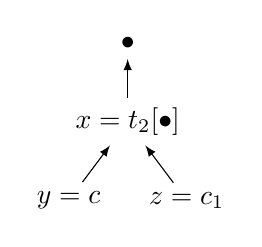
\begin{tikzpicture}[ 
  edge from parent path={(\tikzchildnode\tikzchildanchor) edge [-latex] (\tikzparentnode\tikzparentanchor)},
  level distance=1cm
]
\node (d) {$\bullet$} child{node (a) {$x=t_2[\bullet]$} child{node (b) {$y=c$}} child{node (c)
{$z=c_1$}}};

\end{tikzpicture}
\end{center}
Now each of the environments is represented by a linked list, with the binding
of $x$ shared between them. This is an example of a \emph{shared} environment
~\cite{appel1988optimizing}. This shared, linked structure dates back to the 
first machine for evaluating expressions: Landin's SECD
machine~\cite{landin1964mechanical}.

The drawbacks and advantages of each approach are well known. With a flat
environment, variable lookup can be performed with a simple offset
~\cite{jonesstg,appel2006compiling}. On the other hand, significant
duplication can occur, as we will discuss in Section~\ref{sec:exist}.
With a shared environment, that duplication is removed, but at the cost of
possible link traversal upon dereference. 

As with most topics in compilers and abstract machines, the design space is
actually more complex. For example, Appel and Jim show a wide range of hybrids
~\cite{appel1988optimizing} between the two, and Appel and Shao
~\cite{shao1994space} show an optimized hybrid that aims to achieve the benefits
of both approaches. And as shown in the next section, choice of evaluation
strategy further complicates the picture.

\subsection{Existing Call-by-Need Environments} \label{sec:exist}

Existing call by need machines use flat environments with a heap of
closures~\cite{jonesstg,TIM,johnsson1984efficient,boquist1997grin}. These
environments may contain some combination of primitive values and pointers into the
heap ($p$ below). The pointers and heap implement the memoization of results
required for call by need. Returning to the earlier example, $(\lambda
x.(\lambda y.t) (\lambda z.t_1)) t_2$, we can view a simplified execution state
for this approach when entering $t$ as follows:

\begin{center}
\textbf{Closure}
\begin{align*}
t[x=p, y=p_1] \\
\end{align*}
\textbf{Heap}
\begin{align*}
p &\mapsto t_2[\bullet] \\
p_1 &\mapsto \lambda z.t_1[x=p] 
\end{align*}
\end{center}

If $t_2[\bullet]$ is not in WHNF (this sort of unevaluated closure is called a
\emph{thunk}~\cite{ingerman1961way,peyton1992implementing}), then if it is
entered in either the evaluation of $t$ or $t_1$, the resulting value will
overwrite the closure at $p$. The result of the computation is then shared with
all other instances of $x$ in $t$ and $t_1$. In the case that terms have a large
number of shared variables, environment duplication can be expensive.
Compile-time transformation ~\cite{peyton1992implementing} (tupling arguments)
helps, but we show that the machine can avoid duplication completely.

Depending on $g$, either or both of the closures created for its arguments may
not be evaluated.  Therefore, it is possible that the work of creating the
environment for that thunk will be wasted. This waste is well known, and
existing approaches address it by avoiding thunks as much as possible
~\cite{jonesstg,johnsson1984efficient}. Unfortunately, in cases like the above
example, thunks are necessary. Indeed, even if we tuple the closures for $x$,
$y$, and $z$, that tuple could be wasted if neither $t$ nor $t'$ is used. Thus,
we would like to minimize the cost of creating such thunks.

Thunks are special in another way.  Recall that one advantage of the flat
environments is quick variable lookups. In a lazy language, this advantage is
reduced because \emph{a thunk can only be entered once}. After it is entered, it
is overwritten with a value, so the next time that heap location is entered it
is entered with a value and a different environment. Thus, the work to ensure
that the variable lookup is fast is used only once. This is in contrast to
a call by value language, in which every closure is constructed for a value,
and can be entered an arbitrary number of times. 

A more subtle drawback of the flat environment representation is that
environments can vary in size, and thus a value in WHNF can be too large to fit
in the space allocated for the thunk it is replacing. This problem is discussed
in~\cite{jonesstg}, where the proposed solution is to put the value closure in
a fresh location in the heap where there is sufficient room. The original
thunk location is then replaced with an indirection to the value at the freshly
allocated location. These indirections are removed during garbage collection,
but do impose some cost, both in runtime efficiency and implementation
complexity~\cite{jonesstg}.

We have thus far ignored a number of details with regard to current
implementations. For example, the STG machine can split the flat environment, so
that part is allocated on the stack and part on the heap.  The TIM allocates its
flat environments separately from its closures so that each closure is a code
pointer, environment pointer pair~\cite{TIM} while the STG machine keeps
environment and code co-located~\cite{jonesstg}. Still, the basic design
principle holds: a flat environment for each closure allows quick variable
indexing, but with an initial overhead.

To summarize, the flat environment representation in a call by need language is
whenever a term might be needed, the necessary environment is constructed from
the current environment.  This operation can be expensive, and it is wasted if
the variable is never entered. In this work, we aim to minimize this potentially
unnecessary overhead.

Figure~\ref{fig:designspace} depicts the design space relevant to this paper.
There are existing call by value machines with both flat and shared
environments, and call by need machines with flat environments. As far as we are
aware, we are the first to use a shared environment to implement lazy
evaluation.

\begin{figure*}
\begin{tabularx}{\textwidth}{l | X | X}
                & Flat Environment     & Shared Environment \\ \hline
  Call by need  & STG~\cite{jonesstg}, 
                  TIM~\cite{TIM}, 
                  GRIN~\cite{boquist1997grin} 
                & $\mathcal{CE}$ Machine (this paper) \\
  Call by value & ZAM~\cite{leroy1990zinc}, 
                  SML/NJ~\cite{appel1991standard}
                & ZAM,
                  SECD~\cite{landin1964mechanical}, 
                  SML/NJ \\
\end{tabularx}
\caption{Evaluation strategy and environment structure design space. Each
acronym refers to an existing implementation. Some implementations use multiple
environment representations.}
\label{fig:designspace}
\end{figure*}

\subsection{Big Step Semantics}

Our big step semantics closely resemble the standard call-by-need semantics,
with a few changes for one purpose: instead of standard lambda terms, we now are
using terms with deBruijn indices, and closing the the lambda term under a
pointer into a shared environment structure.  

The big step semantics can be seen in Figure~\ref{fig:bigstepcem}. The
\texttt{clu} function is a partial function that looks up a closure in the
shared environment. Here we use a direct function, but later this will be
replaced by a relation, as it will clearly take a non-constant number of
instructions to execute. Our abstraction rule is identical to the call-by-name
case, and the application rule evaluates the left hand side, then binds the
argument closure to a fresh location in the heap, which extends the environment
of the function computed on the left hand side. Then if the body with this
extended environment evaluates to a value, then the application as a whole
evaluates to a value.

We define a cactus environment machine state to be well formed if, like the
call-by-name semantics, a closure bound in the heap is closed to the left.
We also require the closure in question to be closed under the reachable heap,
and all domain variables to be unique across both the unreachable and reachables
heaps. Because we are using deBruijn indices, when referring to a fresh heap
location, we don't require freshness with respect to a substitution term,
because there is no substitution. This will be important when relating the two
states. We have the following lemma showing that well-formedness is preserved
through evaluation: 

\begin{lstlisting}
Lemma well_formed_step : ∀ c v, well_formed c → c ⇓ v → well_formed v.
\end{lstlisting}

This proof proceeds by induction on the step relation. For the \texttt{Id} rule,
it follows from the fact that the current closure is closed under the reachable
heap, so that we may safely insert it into a location in the unreachable heap
while retaining that it stays closed under the heap to the left. In addition, we
can take a closure from somewhere in the reachable heap, and safely shift our
reachable heap over to the left of that closure while making that closure our
current closure, corresponding to entering a closure. Note that because we
inform.     

\begin{figure}
\begin{lstlisting}
Inductive step : configuration → configuration → Prop :=
  | Id : ∀ M B x y z Φ Φ' Υ Ψ v e, clu v z (Υ ++ x↦cl M y::Φ) = Some (x, M) → 
      ⟨Φ & x↦cl M y, Υ, Ψ⟩M ⇓ ⟨Φ' & x↦cl M y, Υ, Ψ⟩close (:λB) e →
    ⟨Φ, x↦cl M y, Υ & Ψ⟩close v z ⇓ ⟨Φ', x↦ cl (close (:λB) e) y, Υ & Ψ⟩close (:λB) e
  | Abs : ∀ N Φ Ψ e, ⟨Φ & Ψ⟩close (:λN) e ⇓ ⟨Φ & Ψ⟩close (:λN) e
  | App : ∀ N M B B' Φ Φ' Ψ Υ f e ne ae, 
                  f ∉ domain (Ψ ++ Φ') → 
          ⟨Φ & Ψ⟩close M e ⇓ ⟨Φ' & Ψ⟩close (:λB) ne → 
      ⟨Φ', f ↦cl (close N e) ne & Ψ⟩close B f ⇓ ⟨Υ & Ψ⟩close (:λB') ae   →
              ⟨Φ & Ψ⟩close (M@N) e ⇓ ⟨Υ & Ψ⟩close (:λB') ae
where " c1 '⇓' c2 " := (step c1 c2).
\end{lstlisting}
\caption{Big Step Semantics for $\mathcal{CE}$}
\label{fig:bigstepcem}
\end{figure}



\section{Cactus Environment Small Step Semantics}

This section describes how we define small step semantics using a stack to track
argument closures from the \texttt{App} rule and update markers from the
\texttt{Id} rule. By defining this intermediate semantics, we ease the proof
burden between the big-step semantics and the assembly machine semantics.   

\subsection{Semantics}

The rules for our small step semantics closely map to the rules of of the big
step semantics. We split the Id and App rules into rules that push and pop off
the stack. The \texttt{Id} rule gets split into the \texttt{Update} and
\texttt{Var'} rules, which take an update marker and replace the closure at that
location with the current value, and push an update marker, respectively. 

One major difference is that we have to drop the reachability requirement here.
Because we have no way to \emph{remember} the reachability ordering without
pushing something onto the stack, we must change our heap to be a monolithic
single heap, and then reason about the existence of a partitioning of the heap
to be equivalent to the big step semantics. This is analagous to a kind of
\emph{erasure} of information about reachability. It does raise questions as to
whether or not there is some way to retain this information for a cheap way to
re-allocate memory, but that is beyond the scope of this work.

Our well formed property for the small step semantics is a bit different, due to
the monolithic heap. We don't actually require any well-formedness property for
the stack, though investigating that possibility would make for interesting
future work. That said, the proof of retention of well-formedeness is much
simpler: there is no inductive step.   

\begin{figure}
\begin{lstlisting}
Inductive step' : state → state → Prop :=
  | Upd : ∀ Φ Υ Ψ b e e' c l s, 
  st Ψ (Φ++(l,cl c e')::Υ) (inr l::s) (close (lam b) e) →s 
  st Ψ (Φ++(l,cl (close (lam b) e) e')::Υ) s (close (lam b) e)
  | Var' : ∀ Υ Φ Ψ s v l c e e', 
  clu v e (Φ++(l,cl c e')::Υ) = Some (l,c) → 
  st (Φ++(l,cl c e')::Υ) Ψ s (close (var v) e) →s 
  st Υ (Ψ++Φ++[(l,cl c e')]) (inr l::s) c
  | Abs' : ∀ Υ Φ b e f c s, 
  f ∉ domain (Υ ++ Φ) → 
  st Υ Φ (inl c::s) (close (lam b) e) →s 
  st ((f, cl c e)::Υ) Φ s (close b f)
  | App' : ∀ Υ Φ e s n m, 
  st Υ Φ s (close (app m n) e) →s 
  st Υ Φ (inl (close n e)::s) (close m e)
where " c1 '→s' c2 " := (step' c1 c2).
\end{lstlisting}
\caption{Small Step $\mathcal{CE}$ Semantics}
\end{figure}

\subsection{Relation to Big Step $\mathcal{CE}$ Semantics}

We prove that the cesm implements the big-step semantics and the reflexive
transitive closure of the small-step semantics. The relation itself is generally
uninteresting; the heap structure is essentially the same so we require equality
of the heap and concatenation of the big step heaps, and we require nothing of
the stack. Furthermore, the terms and closures are equivalent. Really, the only
goal of this proof is to show that the stack preserves the computation
structure.  

\begin{lstlisting}
Lemma bigstep_smallstep : ∀ c h v h' s, 
  big.step (big.st c h) (big.st v h') → 
  refl_trans_clos small.step (small.st c s h) (small.st v s h')
\end{lstlisting}

Note that the relation is defined on the reflexive transitive closure of the
small-step relation \emph{for all stacks}. We use the fact that this implies
that the same relation will hold for the empty stack, which is the initial and
final state of the small-step machine, as desired.


\section{Machine Code}

In this section we describe the machine semantics, and how the relation with the
stack machine from the previous section works. We can then write down the full
relation to the natural semantics of the source by composing this relation with
the big-step to small-step relation. We thus end up with our final proof, namely
that the call-by-need semantics are preserved by the machine semantics. 

\subsection{Machine Semantics}

The machine semantics are what one would expect given the instructions and
machine state. We omit the full semantics, though they are available in the
source Coq files.

Some of the less obvious semantics: a closure is represented as two machine
words, or \texttt{nat}s in our case. The first is an instruction pointer. The
second is an environment pointer pointing into the heap. Our current closure is
defined by our instruction pointer and environment pointer registers. 

On the stack, we differentiate between update markers and argument closures by
using a zero in place of an instruction pointer, therefore disallowing a zero
instruction pointer, in agreement with modern conventions. We can then check for
zero on the top of the stack, and in the case of This allows for  

\subsection{Relation with Small Step $\mathcal{CE}$ Semantics}

We define our relation on the basic blocks created by the compiler. We relate
the machine and small step states in fairly simple ways. The deBruijn terms of
the small step semantics are all replaced with pointers into instruction memory,
and we require that the mapping preserved compilation equivalence. 

For execution of instructions, we relate each rule in the small step semantics
to a basic block of code. Note that we've artificially increased the number of
instructions in this case and could trivially show that a sound optimization
removing all of the unconditional \texttt{jmp} instructions to the next
instruction. 

In the same way substitution is often modeled as a single step, when
implementing the lookup in the machine semantics we must convert our
\texttt{clu} to a an inductive lookup executed by machine instructions. Of
course, this takes a number of instructions proportional to the size of the
deBruijn index. 

Our heap relation is fairly straightforward. Each cell of the $\mathcal{CE}$
semantics corresponds with three machine words: for the closure there will be an
instruction pointer and an environment pointer, and then one machine words for
the environment continuation. A cell is equivalent to one of these triplets iff
the instruction pointer points to a basic block that is equivalent to the term,
and the environment pointers are equivalent modulo heap location isomorphism.

Note that we do require that the \texttt{new} instruction returns a block of
machine words. This is in contrast to flat representations, where it needs to
return blocks of variables sizes. This is also a situation in which the
simplicity of the $\mathcal{CE}$ machine is very valuable: because of this
constant sized closures, we don't need to worry about cases in which the
value closure that we update a heap location with has more free variables, and
therefore requires more space, leading to the need for indirections as in the
STG machine \cite{STG}.



\section{Applications}

Now that we've seen how the compiler preserves the semantics of the source
language, we can look at what sorts of tools this gives us for reasoning about
the output of the compiler. The basic idea is as follows: because of the
strength of the bisimulation relation, almost all reasoning about the source
semantics is preserved through to the resulting binary. This includes properties
like runtime, heap usage, stack size, types, and of course, correctness of
the results.

\subsection{Time}

One of the most common concerns for someone writing source code for a compiler
is runtime. The ability of programmers to reason about their code's performance
is hampered by the common philosophy of compilers: use any means necessary, no
matter how hard to reason about at the source level, to make code run fast. This
is a reasonable default; when reasoning about code performance, it is a very
rare case that the programmer \emph{doesn't} want their code to run as fast as
possible. 

That said, there are cases when the compiler isn't clever enough. The long-lived
hope for the \emph{sufficiently clever compiler} is dead. Instead, programmers
are forced to rewrite their code to improve performance. Re-writing code to
improve performance will often require reasoning about opaque decisions made by
an optimizing compiler; not an easy task by any measure.

For example, a canonical example of beautiful Haskell code is the efficient
implementation of the fibonacci sequence: 

\begin{lstlisting}[language=Haskell]
fibs = 1:1:zipWith (+) fibs (tail fibs)
\end{lstlisting}

Because Haskell is technically a non-strict language, we rely on our compiler to
"make the right choice" and implement the above \texttt{fibs} using
call-by-need, as using call-by-name would result in exponential complexity.
Relying on opaque decisions like this, when the difference is
\emph{exponential}, is problematic, and makes reasoning about code performance
in a reliable way impossible. We argue that with a verified compiler with a
fixed semantics we improve the programmers ability to reason formally about
performance. 

Towards this goal, we present a theorem allowing the programmer to reason
formally about the time, in number of instructions, that the computation will
take. Of course, number of instructions is a mediocre-at-best approximation of
time, but it will at least prevent any asymptotic surprises, like the
\texttt{fibs} case above. To do this

\subsection{Types}

When we discuss reasoning about our programs at the source level, it would be
irresponsible to give types anything less than their own subsection. Types are
how we do formal reasoning about programs in practice, and when building a
compiler, we'd like to make sure this reasoning is preserved to machine code.
Chlipala showed elegantly how types can be provably preserved through
compilation of simply typed strict lambda calculus in \cite{?}. While this paper
has focused on untyped lambda calculus, we use this section to show how the
strength of the bisimulation proof ensures that any type-based reasoning will be
preserved through evaluation.  

Unfortunately, because we've already fixed our term syntax to be untyped, we
cannot do this reasoning within the common context of explicitly typed
langauges, e.g. System F or the Calculus of Constructions. Instead, we must turn
to a completely implicit type system, which makes type judgements on simple
lambda terms, not unlike a subset of existing Hindley-Milner style languages. We
see no reasoning that this line of reasoning should not extend to more powerful
explicit type systems. 

To formalize this, we generalize the notion of a type judgement to any relation
between a source term and some arbtrary type, represented as a Type variable in
Coq. Leaving the type system completely abstract, we define a typing judgement
to be of the form:

\begin{lstlisting}
Variable type : Type.
Variable hasType : relation tm type.
\end{lstlisting}

To reason about our abstract type we turn to a property that just about every
type system must ahere to: preservation. Preservation says that if a term has a
type, and takes one or more steps, its type must be preserved. We choose to
define preservation using the semantics of call-by-name, as they are our
simplest semantics when to use when we aren't concerned with operational
subtleties.

\begin{lstlisting}
Variable preservation : ∀ (t t':tm) (tau:type), 
  hasType t tau → 
  cbname.step t t' →
  hasType t' tau.
\end{lstlisting}

Given a proof of presevation for our type system for call-by-name, we can prove
that the compiled code respects this, similar to Chlipala's proof that his
simply typed lambda calculus compiler was type-preserving \cite{?}.

\begin{lstlisting}
Theorem assembly_preserves : ∀ t tau p s v, 
  hasType t tau → 
  compiles t p → 
  executes p s →
  term_machine_state_rel s v → 
  hasType v tau.
\end{lstlisting}

In words, this means that if our source term has type \texttt{tau} and
succesfully compiles (likely that typechecking would imply succesful compilation,
but we don't require it), and the compiled program \texttt{p} evaluates to some
machine state \texttt{s}, then any term related by our bisimulation relation
will also have type \texttt{tau}.

\subsection{Space}

Reasoning about space usage in lazy languages is notoriously difficult.
Optimization decisions like deforestation can have effects on the
\emph{asymtotic} memory consumption, making attempts to formally bound memory
consumption impractical at best. 

Generally there are two ways space computations can fail: the one we will focus
on currently is stack overflow. Stack overflows occur when the maximum allocated
stack space is exceeded. This kind of failure is ubiquitous and hard to reason
about. It is the cited cause of failures and even deaths in the case of Toyota's
unintended acceleration case. We show how using the bisimulation proof, we can
prove that stack overflows won't happen given an input program. 

Reasoning about heap space is a bit more difficult currently. This is
because we build on the call-by-need semantics that ensures variables are fresh
with respect to the \emph{entire} heap domain. There are a few ways around this.
One would be to incorporate the notion of a garbage collector as an intermediate
step between reduction steps. A more elegant approach, and that taken by
Chlipala~\cite{chlipala}, is to relax the freshness constraint to be only fresh
with respect to \emph{reachable} heap locations. In this way, we get a more
direct way of reasoning about space usage. With some tools to reason about space
usage at the source level, we could then ensure that this class of reasoning
about heap space is preserved through to the machine code.

\subsection{Programs that \emph{Really} Can't Go Wrong}

Typed functional language programmers often lean on the fact that their programs
"can't go wrong". This important property of typed functional languages is
hampered by an asterisk: "unless it runs out of memory".  The previous sections
on formal reasoning about time and space requirements using this verified
compiler provide an exciting area for future research: removing this asterisk.
In this way, we take a step towards programs that \emph{really} don't go wrong;
they provably won't run out of space or time. This is incredibly useful for many
domains, where these resources are constrained, but we would still like
correctness properties to hold. For example, in the Toyota case above, a proof
that the stack stayed within its bounds could have potentially even saved lives.
This approach also allows us to specify bounds on number of instructions, as
there are many cases in which the number of instructions before a computation
completes is strictly bounded, e.g. heart monitors, video games, etc. A
microcontroller in a car that has a proof that "when it terminates, it will do
the right thing", is of little use.  

Essentially, this ability to broaden the sense in which programs "can't go
wrong", and prove that these properties are preserved through compilation is an
exciting area that this paper takes a step towards. Of course, there is still
much work to be done, as reasoning about these properties even at the source
level is incredibly difficult.



\section{Discussion}

Now that we've covered how the verified compiler works, and gone over some of
the ways which we can utilize the the verification, we use this section to
discuss threats to validity, future work, and related work. 

\subsection{Threats to Validity}

One threat common to all machine-verified work is the verification of the
verifier. This paper has the special position insofar as it could lend itself to
the verification of Coq itself. One of the requirements for verifying that Coq
itself is correct is verifying that the evaluation/reduction of Coq terms is
correct. While full Beta reduction is often employed, weak noramalization
methods such are also employed \cite{?}.  

Another potential qualm with this paper would be that we haven't presented any
performance numbers. That is to say, we have given no evidence that the
performance of this abstract machine isn't abysmal. For that, we point to
previous work \cite{?}, showing that with some extra effort, there's a chance
that this approach could perform at the level of optimizing compilers such as
GHC. That said, we don't plan to implement the barrage of optimizations that
standard compilers employ. Instead, we aim to give the programmer tools to
\emph{reason} about performance of the resulting code, something that many
optimization passes inhibit with the goal of producing fast code at any cost. 

A third threat to validity is with regards to our claim that one can "reason
about performance". In fact, we have only given tools to reason about \emph{number of
instructions}, which is a meager approximation of performance at best.
Unfortunately, hardware is so sophisticated and opaque that full reasoning about
performance is impossible. Features like sophisticated branch prediction,
proprietary memory controllers, etc. prevent any formal reasoning about actual
number of cycles to perform a computation.  

Another worrying aspect of this paper is that any reasoning about time and space
requirements of the assembly code is dependent on reasoning about the big step
semantics of call-by-need, which is notoriously difficult. We admit to this as a
weakness of the current paper, and discuss the need for tools for reasoning
about lazy time and space requirements in the next subsection.

\subsection{Future work}

There are many aspects of the paper that beg further work. One obvious one is to
close the gap between the abstract assembly machine and actual hardware
implementations such as x64, ARM, and MIPS. A valuable addition to this line of
work would be a proper register allocator; something which this work does not
address. A third avenue in thes vein would be to add IEEE primitive literals and
operations to the language, as done in \cite{?}, and verify their correctness.

As mentioned in the previous subsection, while this work gives formal ability to
reason about performance of the resulting code, it requires reasoning about
call-by-need semantics to do so, which is challenging at best, nigh impossible
at worst \cite{?}. We that this problem is made even worse by optimizing
compilers for lazy languages, like GHC. Indeed, optimizations like the
full-laziness-transformation can lead to worse-performing code. A verified
compiler like this one presents the opportunity to verify rewrite rules and
optimizations, potentially in a way that preserves some specified source
language semantics. For example, if some form of substructural type system was
utilized, e.g. linear types, one could reason about optimizations dependent on
linear types at the source level and have that reasoning be preserved through to
machine code.

A third exciting area for future work is the implementation of \emph{verified
optimizations}. Because have have the ability to reason about the effect that
any transformation will have on the number of machine instructions that will be
executed, we can reason about when an optimization is \emph{gauranteed} to
improve performance. As mentioned above, there are existing "optimizations" that
occasionally hurt performance. A verified compiler provides a framework in which
we can verify that our optimizations will never hurt performance. 


\subsection{Related Work}

Here we'll focus mostly on how this work relates to other verified compilers. In
a sense, the job is an easy one: all other verified compilers of functional
languages differ in two important ways: 

\begin{itemize}
\item They are implemented for strict languages
\item They only prove correctness of results, not correctness of process to get
results
\end{itemize}

The two points are related. As we suggested earlier, while for a strict language
there aren't any reasonable operational semantics that have disastrous
consequences for runtime. In contrast, non-strict languages have two perfectly
reasonable implementations, call-by-name and call-by-need, where call-by-name is
often exponentially slower than the call-by-need, as in the \texttt{fibs}
example given earlier. For this reason, it's important to verify the asymptotic
performance of our compiler, and we therefore guarantee that it implements
call-by-need. 

For these reasons, all existing works only verify the results of a computation.
Chlipala has shown that verified compilation can preserve types and semantics
through transformations such as CPS \cite{chlipala}. Chlipala has also shown
that one can add mutable references and exceptions to achieve a verified
compiler for an impure functional language \cite{chlipalaimpure}.  

There has also been some recent work on unverified reasoning about time and
space requirements for a compiler. Hoffman et al. show how to automatically
compute polynomial resource bounds for first order programs
~\cite{hoffmanresource}. 



\section{Conclusion}

We have shown how to build a verified compiler using bisimulation that verifies
time and space requirements in addition to the usual correctness properties. We
have used this technique to build a verified compiler of call-by-need, proving
that the memoization of results is implemented correctly. This is the first
machine-checked proof that an optimization is \emph{preserved through
compilation} that we are aware of. While we haven't proved that the memoization
of results is a true optimization, and it likely isn't in general, we have built
a framework where that sort of reasoning is possible, a significant achievement. 

Typed functional language programmers have long leaned on the important property
that their programs "can't go wrong". Historically this property must always
include an important asterisk: "unless it runs out of memory". Without tools to
reason formally about memory usage this asterisk is impossible to confront. We
have shown how one can reason formally about properties like stack size and heap
size, in a way that is preserved to machine code, enabling programmers to
finally manage this wart.



\section{Acknowledgments}
Sandia is a multiprogram laboratory operated by Sandia Corporation, a Lockheed Martin Company, for the United States Department of Energy’s National Nuclear Security Administration under contract DE-AC04-94AL85000.

% We recommend abbrvnat bibliography style.
\bibliographystyle{abbrvnat}
\bibliography{annotated}

\end{document}
